\documentclass[11pt,a4paper]{article}

\usepackage[margin=2.7cm]{geometry}
\usepackage{amsmath,amssymb,amsthm}
\usepackage{bm}
\usepackage{booktabs}
\usepackage{array}
\usepackage{tikz}
\usetikzlibrary{arrows.meta,positioning}
\usepackage[colorlinks=true,linkcolor=blue!50!black,urlcolor=blue!50!black]{hyperref}
\usepackage{enumitem}
\usepackage{microtype}

% --- macros ---
\newcommand{\ket}[1]{\left|#1\right\rangle}
\newcommand{\bra}[1]{\left\langle#1\right|}
\newcommand{\braket}[2]{\left\langle#1\middle|#2\right\rangle}
\newcommand{\hard}{\ket{\mathrm{hard}}}
\newcommand{\soft}{\ket{\mathrm{soft}}}
\newcommand{\white}{\ket{\mathrm{white}}}
\newcommand{\black}{\ket{\mathrm{black}}}
\newtheorem{obs}{Observation}
\theoremstyle{remark}
\newtheorem*{punchline}{Punchline}

\title{Notes on David Albert's Lectures on the\\ Foundations of Quantum Mechanics}
\author{Notes from the lecture series, expanded and made self-contained}
\date{August 2026}

\begin{document}
\maketitle

\begin{abstract}
\noindent These notes reconstruct and expand the most striking arguments from David Albert's
lecture series on the foundations of quantum mechanics (closely following his book
\emph{Quantum Mechanics and Experience}). Three threads are covered:
(i) the ``hardness and colour'' box experiments, which establish that quantum
randomness is not ignorance and that superposition is a genuinely new mode of being;
(ii) the EPR argument and a Bell-type theorem showing that the perfect correlations of
entangled pairs cannot be explained by any local pre-assignment of values; and
(iii) a comparison of the main realist responses --- GRW collapse, Bohmian mechanics,
and Everettian many-worlds --- and what each one costs.
\end{abstract}

\tableofcontents

%======================================================================
\section{Setting the stage: hardness and colour}
%======================================================================

Albert's pedagogical device is to strip the spin-$\tfrac12$ degree of freedom of an
electron of all its historical baggage and rename it. Electrons are imagined to have
two binary properties:
\begin{itemize}[nosep]
  \item \textbf{Hardness} $H$: every electron measured for hardness comes out
        either \emph{hard} or \emph{soft};
  \item \textbf{Colour} $C$: every electron measured for colour comes out
        either \emph{black} or \emph{white}.
\end{itemize}
Physically, ``colour'' and ``hardness'' are spin components along two orthogonal axes
(say $S_z$ and $S_x$), but nothing in the arguments below depends on knowing that.
The measurements are performed by \emph{boxes} (think Stern--Gerlach magnets): an
electron enters through one aperture and exits through one of two ports labelled by
the two possible values. Crucially, these measurements are \emph{repeatable}: a
hard electron fed back into a hardness box comes out hard, with certainty, every
time. So the boxes deserve to be called measuring devices.

The empirical facts are these: hardness and colour are statistically independent
(a white electron is 50/50 hard/soft, and vice versa), and --- the interesting part ---
they are \emph{incompatible}, in the following precise operational sense.

%======================================================================
\section{Observation 1: measuring colour scrambles hardness}
%======================================================================

\begin{obs}
Take an electron and pass it through a hardness box; select the ones that exit
\emph{hard}. Pass these through a colour box; select the ones that exit
\emph{white}. Pass these through a second hardness box. One might expect
100\% \emph{hard} --- these electrons were, after all, just certified hard.
Instead one finds 50\% hard, 50\% soft.
\end{obs}

\begin{center}
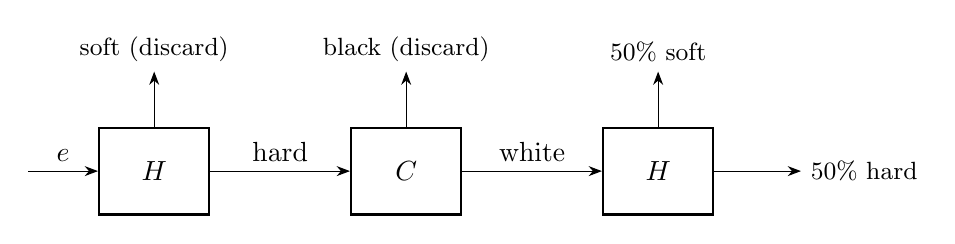
\begin{tikzpicture}[>=Stealth, box/.style={draw, thick, minimum width=1.4cm, minimum height=1.1cm}]
  \node[box] (H1) at (0,0) {$H$};
  \node[box] (C)  at (3.2,0) {$C$};
  \node[box] (H2) at (6.4,0) {$H$};
  \draw[->] (-1.6,0) -- (H1.west) node[midway, above] {$e$};
  \draw[->] (H1.east) -- (C.west) node[midway, above] {hard};
  \draw[->] (C.east) -- (H2.west) node[midway, above] {white};
  \draw[->] (H1.north) -- ++(0,0.7) node[above] {\small soft (discard)};
  \draw[->] (C.north) -- ++(0,0.7) node[above] {\small black (discard)};
  \draw[->] (H2.east) -- ++(1.1,0) node[right] {\small 50\% hard};
  \draw[->] (H2.north) -- ++(0,0.7) node[above] {\small 50\% soft};
\end{tikzpicture}
\end{center}

Measuring colour \emph{scrambles} hardness, and (by symmetry) measuring hardness
scrambles colour. You cannot know both at once. This is just the operational face of
non-commuting observables, but two features of the scrambling deserve emphasis,
because everything later hangs on them.

\paragraph{The statistics are immovable.}
No refinement of the experiment changes the 50/50. You can build the boxes
differently, prepare the electrons differently, select sub-ensembles by any
measurable criterion whatsoever --- \emph{there is nothing one can do to move those
statistics one jot}. This is utterly unlike a coin flip, where the 50/50 reflects
ignorance of initial conditions and a sufficiently obsessive experimenter could
bias the outcome. The quantum 50/50 behaves as if it were a law of nature, not a
confession of ignorance. (Later, Bell's theorem will harden this impression into
a theorem: the outcomes literally could not have been decided in advance by any
local facts about the electron.)

\paragraph{It is not a clumsiness problem.}
The naive gloss --- ``the colour measurement physically disturbs the electron and
knocks its hardness about'' --- turns out to be untenable, and Observation~2 is the
demonstration.

%======================================================================
\section{Observation 2: the two-path experiment}
%======================================================================

\subsection{Recombining the paths undoes the scrambling}

Now build a hardness box whose two output beams are not measured but instead
steered by mirrors into a common region where they are recombined into a single
beam (the recombiner does nothing except bring the paths back together; call the
hard route $P_1$ and the soft route $P_2$). Feed in a \emph{white} electron and
measure the \emph{colour} of what comes out.

\begin{center}
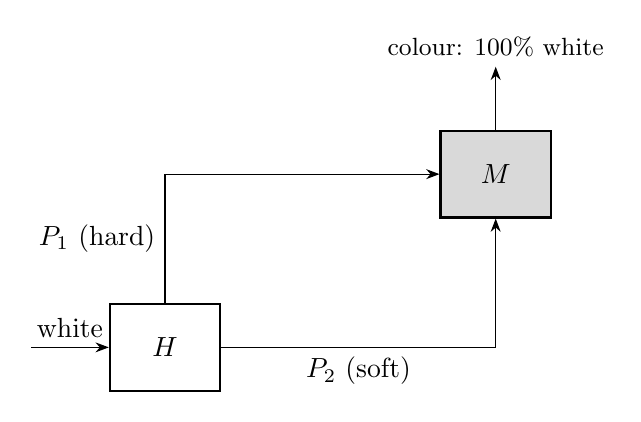
\begin{tikzpicture}[>=Stealth, box/.style={draw, thick, minimum width=1.4cm, minimum height=1.1cm}]
  \node[box] (H) at (0,0) {$H$};
  \node[box, fill=black!15] (M) at (4.2,2.2) {$M$};
  \draw[->] (-1.7,0) -- (H.west) node[midway, above] {white};
  % hard path: up then right
  \draw[->] (H.north) -- (0,2.2) node[midway,left] {$P_1$ (hard)} -- (M.west);
  % soft path: right then up
  \draw[->] (H.east) -- (4.2,0) node[midway,below] {$P_2$ (soft)} -- (M.south);
  \draw[->] (M.north) -- ++(0,0.8) node[above] {\small colour: 100\% white};
\end{tikzpicture}
\end{center}

If the story were ``a hardness measurement disturbs colour,'' then an electron
that took either route through this contraption should have its colour scrambled,
and the output should be 50/50. It is not:

\begin{obs}
Every white electron sent through the recombining device comes out \emph{white},
100\% of the time. The device as a whole does nothing to colour. Hardness ``didn't
scramble colour,'' because the potential paths were made to converge in the same
place.
\end{obs}

But now do anything that determines \emph{which} path the electron took ---
put a detector on one arm, or simply block one arm with a wall --- and the 50/50
scrambling reappears (with a wall in place, half the electrons are absorbed, and the
half that get through are 50/50 black/white). Merely \emph{knowing} the route costs
you the certainty of the output colour.

\subsection{The formalism in two lines}

The two properties correspond to two orthonormal bases of a single two-dimensional
Hilbert space, related by
\begin{equation}
  \white = \tfrac{1}{\sqrt2}\bigl(\hard + \soft\bigr), \qquad
  \black = \tfrac{1}{\sqrt2}\bigl(\hard - \soft\bigr),
  \label{eq:bases}
\end{equation}
(the Born rule then gives all the 50/50s above: e.g.\
$|\braket{\mathrm{hard}}{\mathrm{white}}|^2 = \tfrac12$).
Inside the apparatus, hardness is correlated with route, so a white electron is in
the superposition
\begin{equation}
  \ket{\psi} \;=\; \tfrac{1}{\sqrt2}\bigl(\ket{P_1}\,\hard + \ket{P_2}\,\soft\bigr).
\end{equation}
If the two routes are recombined \emph{coherently} (equal path lengths, no
which-path record anywhere in the universe), the route factors become identical and
drop out, leaving $\tfrac{1}{\sqrt2}(\hard+\soft) = \white$: certainty of white is
restored by \emph{interference} of the two branches. If instead any degree of
freedom ends up correlated with the route --- a detector, a stray photon, a wall ---
the branches can no longer interfere, and each branch alone gives 50/50 colour.
That is what ``measurement scrambles the incompatible property'' really is: not a
mechanical kick, but a destruction of interference.

\subsection{The total-of-nothing box, and the collapse of every which-path story}

Here is the most philosophically loaded step, which the lectures attribute to a
device of Yakir Aharonov's: the \emph{total-of-nothing} (ToN) box. It is a gadget
with the following two \emph{measurable} certifications:
\begin{enumerate}[nosep]
  \item every measurable property of an electron going in equals the corresponding
        property going out --- hardness, colour, energy, everything --- except its
        position in space (it does come out the other side);
  \item the time taken to traverse the box equals the time taken to traverse the
        same stretch of empty space.
\end{enumerate}
By every operational standard, the box does \emph{nothing at all} to an electron
that passes through it. (In the formalism it multiplies the state by $-1$ --- a
phase. A global phase has no measurable consequences whatsoever on a single beam,
which is exactly why the box can pass both certifications.)

Now insert one ToN box into a \emph{single} arm of the recombining device, say the
hard path $P_1$, and again feed in white electrons:

\begin{obs}
With the ToN box on one path, the output is 100\% \emph{black}.
\end{obs}

The one-line calculation: the branch through $P_1$ acquires the factor $-1$,
\begin{equation}
 \tfrac{1}{\sqrt2}\bigl(\ket{P_1}\hard + \ket{P_2}\soft\bigr)
 \;\longrightarrow\;
 \tfrac{1}{\sqrt2}\bigl(-\ket{P_1}\hard + \ket{P_2}\soft\bigr)
 \;\xrightarrow{\ \text{recombine}\ }\;
 \tfrac{1}{\sqrt2}\bigl(-\hard+\soft\bigr) = -\black ,
\end{equation}
and $|{-}1|^2=1$: black with certainty. The phase that was unmeasurable on one beam
is perfectly measurable as a \emph{relative} phase between two beams.

Now run the classic dilemma. A given electron went in white and came out black,
so \emph{something} changed it. Which route did it take?
\begin{itemize}
  \item \textbf{Not $P_1$ alone.} The ToN box demonstrably changes no property of
        any electron that traverses it, and the rest of $P_1$ is empty space.
        An electron travelling only along $P_1$ would have come out white.
  \item \textbf{Not $P_2$ alone.} There is nothing on $P_2$ but empty space; the
        \emph{absence} of a box on your own path can hardly turn you from white to
        black.
  \item \textbf{Not both.} Electrons are never found split; if you look for the
        electron mid-flight you always find the whole electron on exactly one path,
        never fragments on each.
  \item \textbf{Not neither.} Block both paths and nothing comes out at all.
\end{itemize}
Every answer a classical mind can formulate is experimentally refuted. The
electron's mode of travel between the boxes was not ``$P_1$,'' not ``$P_2$,'' not
``both,'' not ``neither.'' It was something for which classical language simply has
no word: a \emph{superposition} of taking $P_1$ and taking $P_2$. Albert's point in
belabouring this is that superposition is not a fancy way of encoding ignorance
about which path was really taken; it is a genuinely novel, experimentally
certified mode of being, and any acceptable interpretation of quantum mechanics
owes us an account of it.

\begin{punchline}
Observation 1 shows quantum statistics are not ignorance about pre-existing
values. Observation 2 shows measurement-disturbance stories fail, and that
``which value/which path'' questions can lack answers altogether. The measurement
problem is then immediate: the linear dynamics that produces these superpositions
should, applied to a measuring device (which is just a big collection of
electrons and nuclei), produce superpositions of \emph{pointer readings} --- yet we
always see one reading. Sections \ref{sec:epr} and \ref{sec:interp} are about the
ways out.
\end{punchline}

%======================================================================
\section{Lecture 4: EPR and a Bell-type theorem}\label{sec:epr}
%======================================================================

\subsection{The setup: perfectly anticorrelated pairs}

There is a preparation protocol $P$ (in real physics: producing two spin-$\tfrac12$
particles in the singlet state) that emits \emph{pairs} of particles, $P_1$ and
$P_2$, which fly apart to two distant laboratories. Each experimenter may measure
any one of three properties $A$, $B$, $C$ on their particle, each with possible
values $\pm1$. (In the concrete realization, $A,B,C$ are spin components along
three coplanar axes $120^\circ$ apart.) The defining empirical fact of the
protocol:
\begin{quote}
If both experimenters measure the \emph{same} property --- $A$ on both, $B$ on
both, or $C$ on both --- the outcomes are \emph{opposite} ($+1$ and $-1$)
100\% of the time.
\end{quote}

\subsection{The EPR argument: locality forces predetermined values}

Suppose \textbf{locality}: nothing you do to $P_1$ can influence $P_2$ once they
are far apart (certainly not faster than light; the measurements can be made at
spacelike separation). Measuring $A$ on $P_1$ then lets you predict with certainty
the value of $A$ on distant $P_2$ --- without touching $P_2$. If the measurement on
$P_1$ cannot have \emph{produced} the opposite value at $P_2$ (that is what
locality forbids), the only remaining explanation of the perfect anticorrelation
is that each particle \emph{already carried} definite values of $A$, $B$, and $C$,
fixed at the source before the particles separated, with the pair anticorrelated
property-by-property. This is the Einstein--Podolsky--Rosen conclusion (1935), in
Bohm's spin version: locality $\Rightarrow$ hidden definite values. Quantum
mechanics, which assigns no such values, would then be an incomplete description.

So far this is coherent --- even attractive. Bell's contribution (1964; the version
below is essentially Mermin's) is that this explanation is not merely
unorthodox but \emph{quantitatively wrong}.

\subsection{What the pre-assigned values would imply}

Suppose each pair leaves the source with definite values. Then each emission is
described by a row of a simple table: $P_1$ carries some triple of $\pm1$'s, and
$P_2$ carries the opposite triple. There are only $2^3 = 8$ possible rows:

\begin{center}
\begin{tabular}{ccc|ccc}
\toprule
\multicolumn{3}{c|}{$P_1$} & \multicolumn{3}{c}{$P_2$}\\
$A$ & $B$ & $C$ & $A$ & $B$ & $C$\\
\midrule
$+1$ & $+1$ & $+1$ & $-1$ & $-1$ & $-1$\\
$+1$ & $+1$ & $-1$ & $-1$ & $-1$ & $+1$\\
$+1$ & $-1$ & $+1$ & $-1$ & $+1$ & $-1$\\
$+1$ & $-1$ & $-1$ & $-1$ & $+1$ & $+1$\\
$-1$ & $+1$ & $+1$ & $+1$ & $-1$ & $-1$\\
$-1$ & $+1$ & $-1$ & $+1$ & $-1$ & $+1$\\
$-1$ & $-1$ & $+1$ & $+1$ & $+1$ & $-1$\\
$-1$ & $-1$ & $-1$ & $+1$ & $+1$ & $+1$\\
\bottomrule
\end{tabular}
\end{center}

Consider the three \emph{mixed} experiments in which the two labs measure
\emph{different} properties: $(A\text{ on }P_1,\,B\text{ on }P_2)$,
$(B\text{ on }P_1,\,C\text{ on }P_2)$, and $(A\text{ on }P_1,\,C\text{ on }P_2)$.
Scan any row of the table and ask: is at least one of these three pairs opposite?
The answer is \emph{yes, in every single row}. The reason is a pigeonhole
argument: among the three values $A_1,B_1,C_1$ carried by $P_1$, at least two must
be equal (three binary values, two slots). Whichever two are equal --- say
$A_1=B_1$ --- the corresponding mixed pair is opposite, since
$B_2=-B_1=-A_1$. Hence, on the hypothesis of pre-assigned local values,
\begin{equation}
  \Pr\bigl[\text{at least one of the three mixed pairs is opposite}\bigr] \;=\; 1
  \qquad\text{(every row, every run).}
  \label{eq:lhv}
\end{equation}

\subsection{What quantum mechanics says}

Quantum mechanics makes a flat prediction for the mixed experiments. For the
singlet state, if the two labs measure spins along axes at angle $\theta$, the
probability of \emph{opposite} outcomes is $\cos^2(\theta/2)$. Same axis
($\theta=0$): probability $1$ --- the perfect anticorrelation we started from.
Different properties, axes $120^\circ$ apart:
\begin{equation}
  \Pr[\text{opposite}] \;=\; \cos^2(60^\circ) \;=\; \tfrac14 .
\end{equation}
Then, by the union bound (probabilities of a union of events cannot exceed the sum),
\begin{equation}
  \Pr\bigl[\text{at least one of the three mixed pairs is opposite}\bigr]
  \;\le\; \tfrac14+\tfrac14+\tfrac14 \;=\; \tfrac34 .
  \label{eq:qm}
\end{equation}
(One cannot measure all three mixed pairs on a single pair of particles, of
course; \eqref{eq:qm} is a statement about the counterfactual values the
local story insists exist, and it is checkable pair-by-pair by choosing the
settings at random.)

Equations \eqref{eq:lhv} and \eqref{eq:qm} contradict each other:
$1 \not\le \tfrac34$. And experiment --- Freedman--Clauser, Aspect, and the 2015
loophole-free tests (2022 Nobel Prize) --- sides with quantum mechanics.

\subsection{What must go}

The pre-assigned values were not an optional flourish; they were \emph{forced} by
locality via the EPR argument. So the conclusion is stark:

\begin{quote}
\textbf{Locality is false.} The correlation between the two outcomes does not
propagate; it does not depend on anything in the space between the labs, and it
does not weaken with distance. And there was \emph{no fact of the matter} about
the outcomes prior to the experiment --- the values are not carried from the
source. The world is, in this specific sense, non-local.
\end{quote}

Note what is \emph{not} implied: no signalling. The local statistics in either
lab are 50/50 regardless of what the other lab does, so the non-locality cannot
be used to communicate. But as an account of what nature is doing, locality in
Einstein's sense is dead.

\paragraph{The many-worlds escape hatch.}
There is exactly one loophole, and Albert flags it repeatedly: the entire argument
presupposes that each measurement has a \emph{unique, determinate outcome} ---
that ``the probability the outcomes were opposite'' refers to something. In the
Everett interpretation this is denied: both outcomes occur, in different branches,
and there is no unique fact of the matter about how the experiments turned out.
The correlations, as single-world facts, simply don't exist; what exists is a
branching structure in which they appear. With that premise removed, Bell's
theorem cannot get started, and many-worlds remains a fully \emph{local} theory.
This is one of its principal selling points --- at a price described below.

%======================================================================
\section{The interpretations: what each one buys and what it costs}\label{sec:interp}
%======================================================================

All parties agree on the phenomena and (in the non-relativistic domain) on the
statistics. They disagree about what is really going on --- in particular about
what happens in a ``measurement,'' given the superposition arguments of
Observation 2. The three realist programmes discussed in the lectures:

\begin{center}
\renewcommand{\arraystretch}{1.35}
\begin{tabular}{>{\raggedright\arraybackslash}p{3.1cm}>{\raggedright\arraybackslash}p{5.1cm}>{\raggedright\arraybackslash}p{6.2cm}}
\toprule
 & \textbf{Pros} & \textbf{Cons}\\
\midrule
\textbf{GRW} (Schr\"odinger evolution + stochastic jumps) &
Solves the measurement problem with explicit, precise dynamics; in principle
empirically distinguishable from standard QM. &
There truly is \emph{no fact of the matter} about uncertain quantities until a
jump occurs; until a big system gets involved, superpositions are ontologically
real. Work needed for a relativistic version. Non-local.\\
\textbf{Bohm} (pilot wave) &
Ontologically conservative: there are only waves and particles; particles always
have definite positions; no collapse, no exotic metaphysics of outcomes. &
The wave lives in $3N$-dimensional configuration space ($N$ = number of particles
in the universe), so the ``wave'' is nothing like a field in 3-space. Work needed
for a relativistic version. \emph{Wildly} non-local.\\
\textbf{Everett} (many worlds) &
Local. Just the Schr\"odinger equation, nothing else --- no collapse, no extra
variables. Generalises to relativistic QFT trivially. &
Unclear what probability means: in what sense can both worlds exist, with
certainty, and yet have different probabilities associated with them?\\
\textbf{Bohr} (Copenhagen) &
--- &
Impossible to tell what the view actually says is going on. The three stories
above are a proof by construction that he was wrong that no such story could be
told.\\
\bottomrule
\end{tabular}
\end{center}

\subsection{GRW: make the collapse real}

Ghirardi, Rimini and Weber (1986) modify the Schr\"odinger equation itself: each
elementary particle has a tiny probability per unit time (about once per
$10^{16}$ s) of undergoing a spontaneous, random localization (``jump'') of its
wavefunction. For one electron in an interferometer this essentially never
happens, so all the interference phenomena of Observation 2 survive. But a
macroscopic pointer contains $\sim 10^{23}$ entangled particles, and one jump
anywhere collapses the whole assembly --- so superpositions of pointer positions
die within microseconds. Measurements have unique outcomes because the dynamics
says so.

The costs, per the lecture: between jumps the superposition is
\emph{ontologically real} --- there is genuinely no fact of the matter about
where the electron is, or which path it takes, until either a jump happens or a
big system gets entangled with it. The theory is explicitly non-local (a jump
here instantaneously reshapes the wavefunction everywhere --- this is how it
accommodates Bell). And making it relativistic is a serious open research
programme, since ``instantaneous collapse'' picks out a preferred frame.
A compensation worth remembering: GRW differs \emph{in principle} from quantum
mechanics (interference of sufficiently large systems is predicted to fail), so
it is a physical hypothesis, not just a reinterpretation.

\subsection{Bohm: particles all the way down}

In Bohmian mechanics (de Broglie 1927, Bohm 1952) there are two things: the
wavefunction, evolving by the Schr\"odinger equation always (no collapse,
ever), and actual point particles with definite positions at all times, whose
velocities are determined by the wavefunction (the ``pilot wave''). The electron
in Observation 2 really does take exactly one path --- but the empty branch of the
wavefunction still travels the other path, and recombines to steer the particle,
which is how the ToN box on the path \emph{not taken} can flip the outcome.
Measurements have unique outcomes because particle configurations are unique;
the 50/50 statistics arise from ignorance of the initial particle positions
(distributed as $|\psi|^2$). This is the ontologically conservative option:
only waves and particles, nothing modal or exotic.

The costs: the ``wave'' is a function on $3N$-dimensional configuration space ---
one axis for every coordinate of every particle in the universe --- so its claim
to be a physical field in space is strained; either you accept a $3N$-dimensional
arena as fundamental or you owe a story about how 3-space emerges. The dynamics
is \emph{wildly} non-local: the velocity of each particle depends
instantaneously on the positions of all the others, however distant (again, this
is how Bell is accommodated, and again it requires a preferred foliation of
spacetime, making a relativistic version hard).

\subsection{Everett: take the Schr\"odinger equation literally}

Everett (1957) keeps the wavefunction and the linear dynamics and adds
\emph{nothing}. When a measuring device interacts with the superposed electron,
the device --- and the experimenter, and the environment --- simply join the
superposition. Decoherence makes the branches dynamically autonomous, and each
branch contains an experimenter who saw a definite outcome. Nothing ever
collapses; ``both things happen.''

The pros are exactly the other theories' cons: the theory is \emph{local} (it
evades Bell by denying unique outcomes, as in \S\ref{sec:epr}); its dynamics is
just the Schr\"odinger equation, with no ad hoc additions; and since it adds no
structure that would conflict with Lorentz invariance, it generalises to
relativistic quantum field theory trivially.

The con is the \emph{probability problem}, and Albert regards it as serious.
Quantum mechanics is confirmed by its statistical predictions --- the Born-rule
frequencies. But in Everett, when you measure the hardness of a white electron,
\emph{both} outcomes occur with certainty. In what sense, then, was the
probability of ``hard'' equal to $\tfrac12$? What are the relative frequencies
evidence \emph{of}, if every run yields every outcome? Unless amplitudes can
be given a genuine probabilistic (or decision-theoretic) role, the very evidence
that supports quantum mechanics seems to be unstatable within the
interpretation. Proposed answers exist (self-locating uncertainty,
Deutsch--Wallace decision theory); whether any succeeds is still contested.

\subsection{Bohr, by way of epilogue}

The Copenhagen position, on Albert's telling, combined two claims: that the
quantum formalism needs no realist story beneath it, and that no coherent such
story is \emph{possible} --- talk of what the electron is doing between
measurements was to be renounced as meaningless. The verdict of the lectures is
blunt: whatever one thinks of GRW, Bohm, and Everett, each is a fully coherent,
empirically adequate account of what is going on --- including during
measurements. They are a \emph{proof by construction} that Bohr was wrong. The
live question in the foundations of quantum mechanics is not \emph{whether} such
a story can be told, but \emph{which} of the tellable stories is true --- and each
candidate exacts a remarkable price: real chancy collapses (GRW), a
$3N$-dimensional pilot wave with radical non-locality (Bohm), or a branching
multiverse in which probability itself needs reconstruction (Everett).

%======================================================================
\section*{Further reading}
%======================================================================
\begin{itemize}[nosep]
  \item D.\,Z. Albert, \emph{Quantum Mechanics and Experience}, Harvard UP (1992)
        --- the book the lectures track; chapters 1--2 are the hardness/colour
        experiments, chapter 3 the EPR/Bell argument.
  \item J.\,S. Bell, \emph{Speakable and Unspeakable in Quantum Mechanics},
        Cambridge UP (2004) --- especially ``Bertlmann's socks and the nature of
        reality.''
  \item N.\,D. Mermin, ``Is the moon there when nobody looks?'', \emph{Physics
        Today} \textbf{38}(4), 38 (1985) --- the version of Bell's theorem used in
        \S\ref{sec:epr}.
  \item T. Maudlin, \emph{Quantum Non-Locality and Relativity}, 3rd ed., Wiley
        (2011) --- what Bell does and does not imply about relativity.
  \item D. Wallace, \emph{The Emergent Multiverse}, Oxford UP (2012) --- the
        state of the art on Everettian probability.
\end{itemize}

\end{document}
